\chapter{Network representation in RSCAD and PowerFactory}

\section{Draft module representation in RSCAD}

\begin{figure}[H]
\centering
%\hspace*{-0.2cm}
    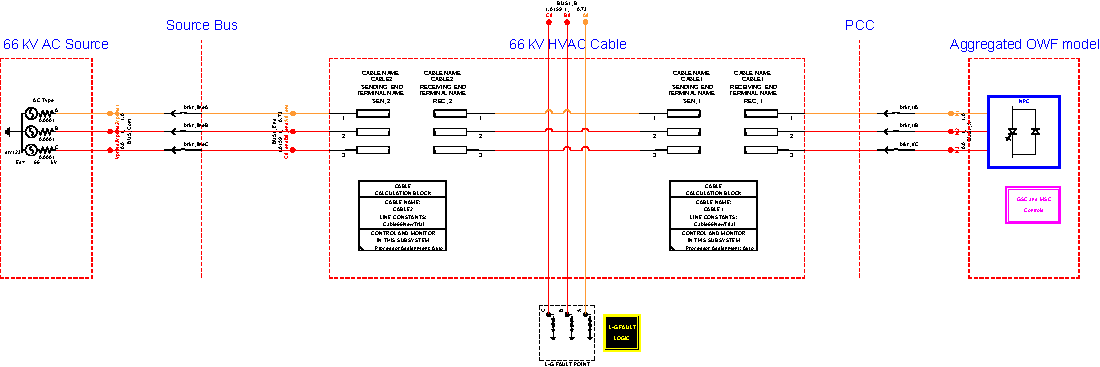
\includegraphics[height = 6cm,width = 17.5cm]{Diagrams/Appendix_B/WT1_AC_RSCAD_network_view.pdf}
    \caption{66 kV HVAC test system representation in Draft module in RSCAD}
    \label{fig:WT1_AC_RSCAD_network_view}
\end{figure}

\section{Runtime module representation in RSCAD}
\begin{figure}[H]
\centering
%\hspace*{-0.2cm}
    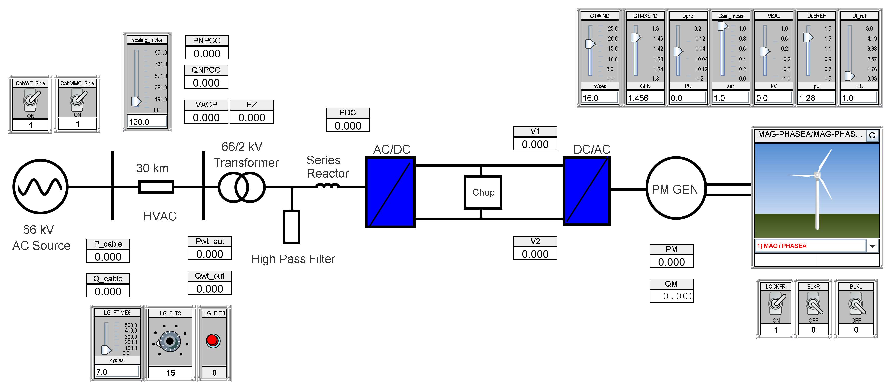
\includegraphics[height = 7cm,width = 16.5cm]{Diagrams/Appendix_B/WT1_AC_RSCAD_network_sib_view.pdf}
    \caption{66 kV HVAC test system representation in Runtime module in RSCAD}
    \label{fig:WT1_AC_RSCAD_network_sib_view}
\end{figure}

\section{Grid overview in PowerFactory}
\begin{figure}[H]
\centering
%\hspace*{-0.2cm}
    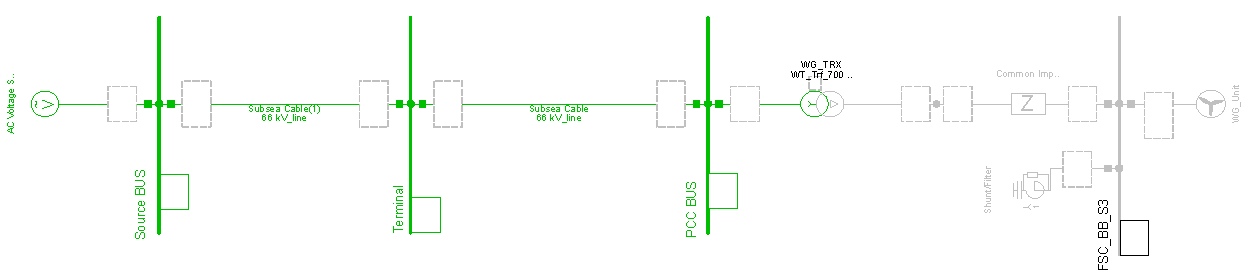
\includegraphics[height = 5cm,width = 17.5cm]{Diagrams/Appendix_B/WT1_AC_PFD_network_view.pdf}
    \caption{66 kV HVAC test system representation in PowerFactory}
    \label{fig:WT1_AC_PFD_network_view}
\end{figure}


\section{Fault logic in RSCAD}\label{fault_logic}
